% ============================================================
%  Proyecto - Analítica y Visualización de Datos
%  Análisis y Visualización de Recetas de Cerveza Artesanal
%  ESCOM - IPN
%
%  Compilar con:  pdflatex main.tex
% ============================================================
\documentclass[11pt]{article}

% ---- Codificación e idioma ----
\usepackage[utf8]{inputenc}
\usepackage[T1]{fontenc}
\usepackage[spanish,es-tabla]{babel}

% ---- Paquetes útiles ----
\usepackage{graphicx}      % imágenes
\usepackage[margin=2.5cm]{geometry}
\usepackage{booktabs}      % tablas bonitas
\usepackage{float}         % posicionar figuras con [H]
\usepackage{caption}
\usepackage{amsmath}       % fórmulas
\usepackage{hyperref}      % enlaces
\hypersetup{colorlinks=true, linkcolor=black, urlcolor=blue}

% ============================================================
%  CARÁTULA
% ============================================================
\begin{document}
\begin{titlepage}
    \centering

    % --- Logos: coloca IPN.png y ESCOM.png en la carpeta logos/ ---
    \begin{minipage}{0.45\textwidth}
        \raggedright
        
\includegraphics[width=2.5cm]{logos/IPN.png}
    \end{minipage}
    \begin{minipage}{0.45\textwidth}
        \raggedleft
        
\includegraphics[width=2.5cm]{logos/ESCOM.png}
    \end{minipage}

    \vspace{1cm}
    {\scshape\large Instituto Politécnico Nacional\par}
    \vspace{0.5cm}
    {\scshape Escuela Superior de Cómputo\par}
    \vspace{0.5cm}
    {\scshape ESCOM \par}
    \vspace{1.5cm}
    {\large Analítica y Visualización de Datos\par}

    \vfill
    {\Huge\bfseries Análisis y Visualización de\\ Recetas de Cerveza Artesanal\par}
    \vfill

    % --- Datos de las integrantes ---
    {\large\bfseries Integrantes:\par}
    \vspace{0.3cm}
    {\large
        Galindo Espinosa Ana Lilia\par
        Herrera Moreno Sayuri\par
    }

    \vspace{0.8cm}
    % TODO: completa estos datos
    {\large Grupo: 5AM1\par}
    \vspace{0.2cm}
    {\large Profesor(a): Alejandro López Gómez\par}

    \vfill
    {\large \today\par}

\end{titlepage}

% ---- Índice ----
\tableofcontents
\newpage


% ============================================================
%  1. INTRODUCCIÓN
% ============================================================
\section{Introducción}
% GUÍA: Presenta el tema en 1-2 párrafos. Responde:
%  - ¿De qué trata el dataset? (recetas de cerveza artesanal, ~73,861 recetas,
%    variables fisicoquímicas como ABV, IBU, color, densidades, etc.)
%  - ¿Por qué es interesante analizarlo?
%  - ¿Qué se va a hacer en este trabajo? (preprocesamiento, similitud,
%    correlación, chi-cuadrada, PCA y un dashboard interactivo)

La cerveza artesanal se elabora siguiendo recetas muy distintas entre sí: algunas
son suaves y ligeras, algunas otras son fuertes, oscuras o demasiado amargas. Cada receta se puede
describir con un conjunto de características numéricas, como su cantidad de alcohol,
su nivel de amargor o su color. Al día de hoy hay muchas recetas disponibles en internet, 
tal cual es el caso del dataset de \textbf{Brewer's Friend} es una comunidad de cerveceros que comparten 
información sobre sus recetas como las que se encuentran en Kaggle,el cual contiene información sobre miles de 
recetas de cerveza artesanal, estilos y métodos de elaboración.

El conjunto de datos utilizado en este análisis reúne más de \textbf{73{,}000 recetas}
de cerveza, cada una con varias de estas características. El problema es que, al tener
tantos registros y tantas variables, resulta muy difícil entender la información
a simple vista. No es fácil saber, por ejemplo, qué estilos de cerveza se parecen
entre sí, qué características están relacionadas (como el alcohol y el azúcar), o si
el estilo de una cerveza tiene que ver con la forma en que se elabora. Además, como
los datos fueron capturados por muchas personas distintas, contienen errores,
valores faltantes y valores fuera de lo normal que deben corregirse antes de
analizarlos.

Por esta razón, en este proyecto se realiza un proceso de limpieza y análisis de los
datos para encontrar patrones y relaciones entre las recetas. Se aplican distintas
técnicas para medir qué tan parecidas son las cervezas entre sí, para identificar
qué características se relacionan, para comprobar si el estilo depende del método de
elaboración y para resumir la información en pocas variables que faciliten su
visualización. Finalmente, los resultados se presentan en un \textbf{tablero
interactivo (dashboard)} que permite explorar la información de forma sencilla.

La descripción detallada del conjunto de datos y el diccionario de variables se
presentan en la siguiente sección.


% ============================================================
%  2. OBJETIVO(S)
% ============================================================
\section{Objetivos}
% GUÍA: Un objetivo general y, si quieres, objetivos específicos en una lista.

\subsection*{Objetivo general}
Analizar y visualizar las características fisicoquímicas de recetas de cerveza artesanal
para identificar patrones, relaciones y agrupamientos entre estilos y métodos de elaboración.

\subsection*{Objetivos específicos}
\begin{itemize}
    \item \textbf{Realizar el preprocesamiento y limpieza del conjunto de datos:}
    corregir los errores presentes en la información, tratar los valores faltantes,
    eliminar los valores fuera de lo normal y dejar los datos en una escala
    comparable, de modo que el análisis posterior sea confiable.

    \item \textbf{Analizar la distribución de las variables fisicoquímicas:}
    observar cómo se comportan variables como el alcohol, el amargor o el color,
    identificando sus valores más frecuentes y su rango.

    \item \textbf{Calcular medidas de similitud entre recetas mediante la distancia
    euclidiana:} determinar qué tan parecidos son los estilos de cerveza a partir
    de sus características, para reconocer cuáles se asemejan más entre sí.

    \item \textbf{Evaluar la correlación entre variables utilizando el coeficiente
    de Pearson:} medir si dos características aumentan o disminuyen juntas, por
    ejemplo, si una mayor cantidad de azúcar inicial se relaciona con más alcohol.

    \item \textbf{Determinar la dependencia entre variables categóricas mediante la
    prueba Chi-cuadrada:} comprobar si el estilo de la cerveza está relacionado con
    el método con el que se elabora, o si son independientes.

    \item \textbf{Aplicar el Análisis de Componentes Principales (PCA):} resumir
    varias variables en unas pocas que conserven la mayor parte de la información,
    para poder visualizar los datos de forma más simple y observar si los estilos
    forman grupos.

    \item \textbf{Desarrollar un dashboard interactivo:} construir una herramienta
    visual que permita explorar la información y los resultados del análisis de
    manera sencilla, sin necesidad de programar.
\end{itemize}


% ============================================================
%  3. DESCRIPCIÓN DEL CONJUNTO DE DATOS
% ============================================================
\section{Descripción del conjunto de datos}

El conjunto de datos utilizado proviene de la comunidad \textbf{Brewer's Friend} y
está disponible en la plataforma Kaggle. Contiene \textbf{73{,}861 recetas} de
cerveza artesanal descritas mediante \textbf{23 columnas}. Cada fila corresponde a
una receta y cada columna a una característica de la cerveza, ya sea numérica (como
el alcohol, el amargor o el color) o categórica (como el estilo o el método de
elaboración).

Dado que la información fue capturada por muchos usuarios distintos, el conjunto
presenta valores faltantes en varias columnas, así como algunos valores fuera de lo
normal que corresponden a errores de captura. Por ello, para este trabajo se
seleccionaron únicamente las variables más relevantes para el análisis
fisicoquímico. En la Tabla~\ref{tab:diccionario} se presenta el diccionario de
datos con el significado de cada variable utilizada.

\begin{table}[H]
    \centering
    \caption{Diccionario de datos: variables utilizadas en el análisis.}
    \label{tab:diccionario}
    \begin{tabular}{lll}
        \toprule
        \textbf{Variable} & \textbf{Significado} & \textbf{Unidad} \\
        \midrule
        ABV        & Cantidad de alcohol de la cerveza               & \%                  \\
        IBU        & Nivel de amargor (aportado por el lúpulo)       & escala IBU          \\
        Color      & Qué tan oscura es la cerveza                    & escala SRM          \\
        OG         & Densidad antes de fermentar (azúcar inicial)    & gravedad específica \\
        FG         & Densidad después de fermentar (azúcar restante) & gravedad específica \\
        Efficiency & Eficiencia del proceso de elaboración           & \%                  \\
        Style      & Estilo de la cerveza (IPA, Lager, etc.)         & categórica          \\
        BrewMethod & Método con el que se elaboró                    & categórica          \\
        \bottomrule
    \end{tabular}
\end{table}


% ============================================================
%  4. METODOLOGÍA
% ============================================================
\section{Metodología}

Para el desarrollo de este proyecto se siguió la metodología \textbf{KDD}
(\textit{Knowledge Discovery in Databases}, o Descubrimiento de Conocimiento en
Bases de Datos), la cual consiste en un proceso estructurado para extraer
información útil a partir de grandes volúmenes de datos. Esta metodología se
compone de las siguientes etapas:

\begin{enumerate}
    \item \textbf{Selección:} se elige el conjunto de datos y las variables
    relevantes para el análisis.
    \item \textbf{Preprocesamiento:} se limpian los datos, tratando valores
    faltantes y valores atípicos.
    \item \textbf{Transformación:} se preparan los datos para el análisis, por
    ejemplo escalándolos a una misma medida.
    \item \textbf{Minería de datos:} se aplican las técnicas de análisis para
    encontrar patrones y relaciones.
    \item \textbf{Interpretación y evaluación:} se interpretan los resultados
    obtenidos para convertirlos en conocimiento.
\end{enumerate}

En este trabajo se aplicó el proceso KDD \textbf{hasta la etapa de análisis de
datos}, ya que el objetivo es comprender, describir y visualizar la información,
y no construir un modelo de predicción. A continuación se describe cada etapa
realizada.

\subsection{Selección y preprocesamiento de datos}

\textbf{Selección.} Del conjunto original de 23 columnas se descartaron aquellas
que solo funcionan como identificadores y no aportan información sobre las
características de la cerveza, como la dirección web de la receta (URL) y el
identificador de usuario (UserId). También se omitieron columnas con una gran
cantidad de valores faltantes. De esta manera, se conservaron las variables
fisicoquímicas de interés (ABV, IBU, Color, OG, FG y Efficiency) junto con las
variables categóricas Style y BrewMethod.

\textbf{Limpieza.} Se eliminaron los registros duplicados. Posteriormente se
revisaron los valores faltantes en las variables seleccionadas; como estas no
presentaban datos ausentes, no fue necesario aplicar ninguna técnica de imputación.

Para los valores atípicos (valores fuera de lo normal, generalmente errores de
captura) se utilizó el \textbf{método del rango intercuartílico (IQR)}. Este método
considera atípico cualquier valor que quede por debajo de $Q_1 - 1.5 \cdot IQR$ o
por encima de $Q_3 + 1.5 \cdot IQR$, donde $Q_1$ y $Q_3$ son el primer y tercer
cuartil. Gracias a este filtrado, el conjunto de datos pasó de \textbf{73{,}861 a
49{,}217 recetas}, eliminando valores claramente erróneos (por ejemplo, niveles de
amargor imposibles para una cerveza real).

\textbf{Transformación.} Finalmente, las variables se \textbf{estandarizaron} con
\textit{StandardScaler}, dejándolas con media cero y desviación estándar uno. Este
paso es necesario porque las variables están en escalas muy distintas (por ejemplo,
el IBU toma valores de varias decenas mientras que la densidad ronda 1.0); sin
estandarizar, las variables de mayor magnitud dominarían los cálculos de distancia
y el análisis de componentes principales.

Una vez preparados los datos, se realizó la etapa de \textbf{análisis de datos},
en la que se aplicaron las siguientes técnicas.

\subsection{Medidas de similitud (distancia euclidiana)}

Para identificar qué estilos de cerveza se parecen más entre sí, se calculó la
\textbf{distancia euclidiana}. Esta distancia mide qué tan separados están dos
puntos: a menor distancia, mayor parecido. Como cada estilo tiene muchas recetas,
primero se obtuvo el \textbf{promedio de cada variable por estilo} (un perfil
representativo de cada estilo) usando los datos ya estandarizados. El análisis se
limitó a los \textbf{15 estilos más frecuentes}, ya que los estilos con muy pocas
recetas no son representativos y dificultan la lectura del resultado. Con estos
perfiles se construyó una matriz de distancias, que se representó mediante un mapa
de calor (\textit{heatmap}).

\subsection{Correlación de Pearson}

Para conocer la relación entre las variables numéricas se utilizó el
\textbf{coeficiente de correlación de Pearson}, que toma valores entre $-1$ y $1$.
Un valor cercano a $1$ indica que dos variables aumentan juntas, uno cercano a
$-1$ que cuando una sube la otra baja, y un valor cercano a $0$ que no existe una
relación lineal. Se calcularon especialmente las relaciones entre el alcohol y el
amargor (ABV--IBU), el alcohol y la densidad inicial (ABV--OG) y el amargor y el
color (IBU--Color).

\subsection{Prueba Chi-cuadrada}

Para comprobar si el estilo de la cerveza depende del método con el que se elabora
se aplicó la \textbf{prueba Chi-cuadrada}, que sirve para analizar la relación
entre dos variables categóricas. Se construyó una tabla de contingencia entre el
estilo (\textit{Style}) y el método (\textit{BrewMethod}). Debido a que existen
muchos estilos distintos, se agruparon en los \textbf{10 más frecuentes} más una
categoría ``Otros'', con el fin de cumplir el supuesto de la prueba, que requiere
que las frecuencias esperadas en cada celda sean suficientes (mayores o iguales a
5).

\subsection{Análisis de Componentes Principales (PCA)}

Para resumir la información se utilizó el \textbf{Análisis de Componentes
Principales (PCA)}, una técnica que combina las variables originales en unas pocas
variables nuevas, llamadas componentes, que conservan la mayor parte de la
información. Se aplicó PCA sobre las seis variables fisicoquímicas estandarizadas
para reducirlas a \textbf{dos componentes}, lo que permite representar las recetas
en una gráfica de dos dimensiones y observar si los estilos forman grupos.

\subsection{Dashboard}

Finalmente, para facilitar la exploración de los datos se desarrolló un
\textbf{dashboard interactivo} utilizando las herramientas \textit{Streamlit} y
\textit{Plotly}. El dashboard cuenta con filtros (por estilo, método y rangos de
alcohol y amargor) que actualizan todas las gráficas de forma automática, así como
indicadores resumen y varias pestañas que organizan la información en distribución
de estilos, histogramas, relaciones entre variables y una tabla de datos.


% ============================================================
%  4. RESULTADOS
% ============================================================
\section{Resultados}

\subsection{Distribución de las variables}

En primer lugar se analizó cómo se distribuyen las recetas según sus estilos y sus
características. La Figura~\ref{fig:estilos} muestra los estilos con mayor número de
recetas, donde destacan claramente las variantes de cerveza tipo \textit{American
IPA} y \textit{American Pale Ale}. Por su parte, las Figuras~\ref{fig:histabv} y
\ref{fig:histibu} presentan la distribución del alcohol (ABV) y del amargor (IBU),
respectivamente; en ambos casos la mayoría de las recetas se concentra en valores
bajos a moderados.

\begin{figure}[H]
    \centering
    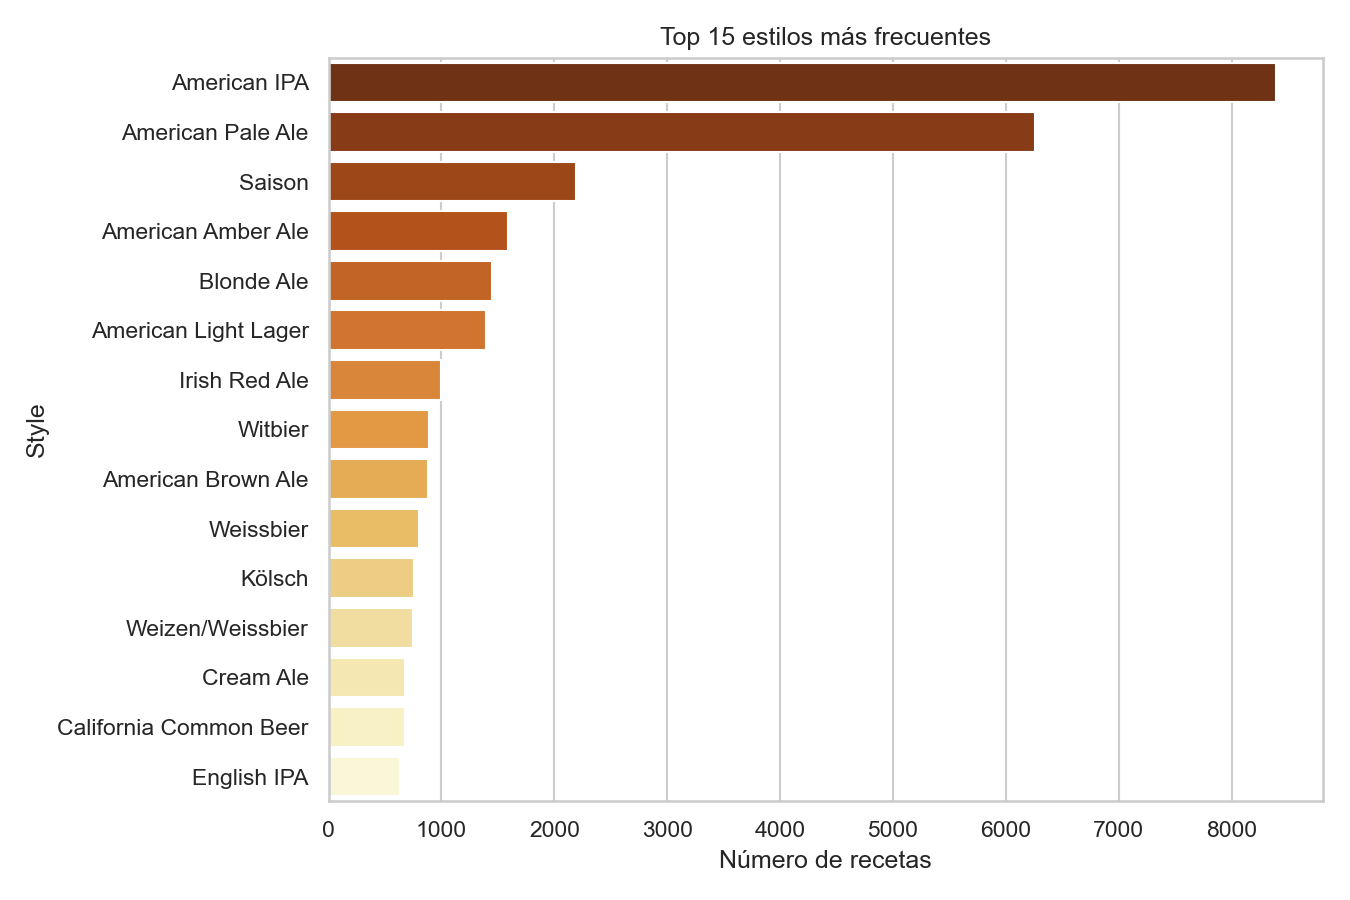
\includegraphics[width=0.75\textwidth]{figuras/dist_estilos.png}
    \caption{Estilos de cerveza más frecuentes en el conjunto de datos.}
    \label{fig:estilos}
\end{figure}

\begin{figure}[H]
    \centering
    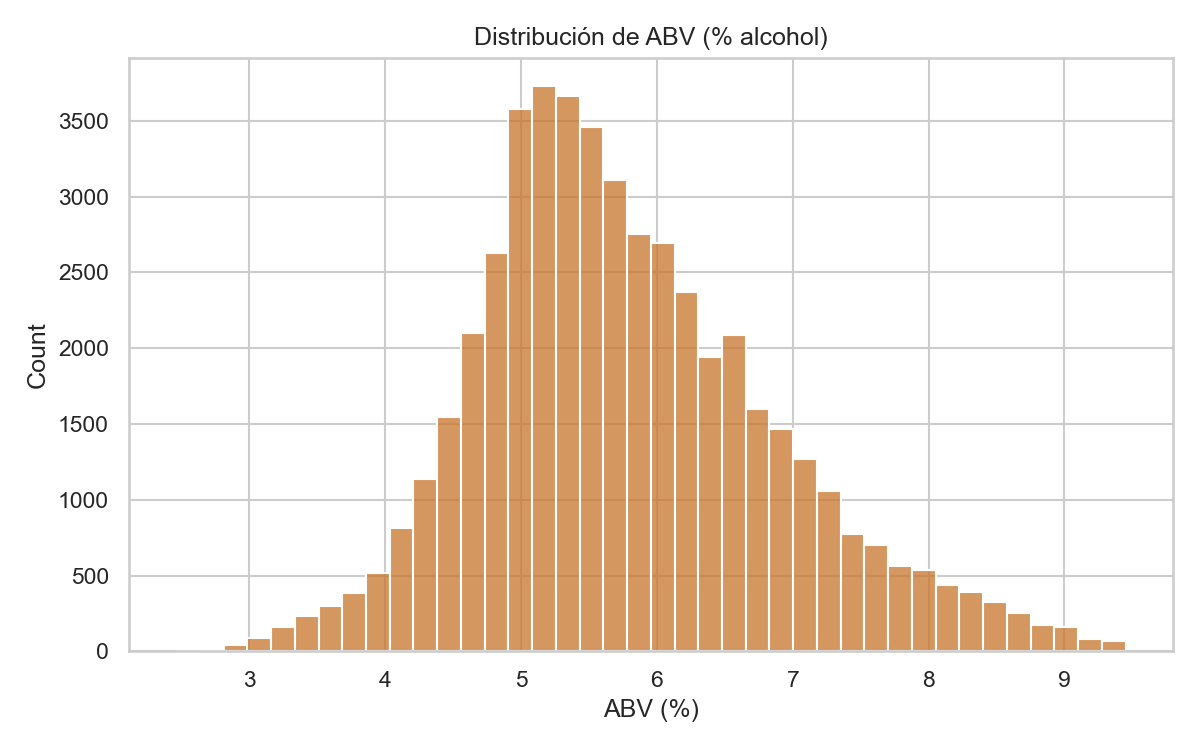
\includegraphics[width=0.49\textwidth]{figuras/hist_abv.png}
    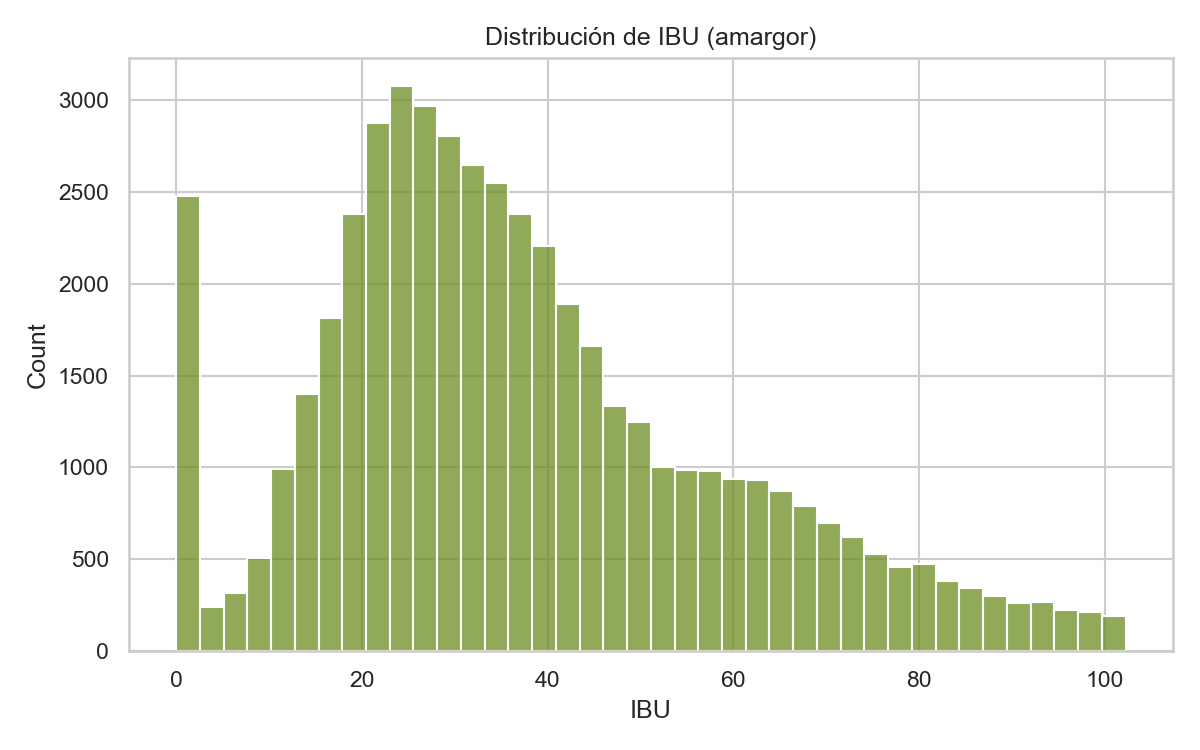
\includegraphics[width=0.49\textwidth]{figuras/hist_ibu.png}
    \caption{Distribución del alcohol (ABV) y del amargor (IBU).}
    \label{fig:histabv}
    \label{fig:histibu}
\end{figure}

\subsection{Similitud entre estilos}

A partir de la matriz de distancias euclidianas (Figura~\ref{fig:heatmap}) se
observa que los estilos más parecidos entre sí son \textbf{Blonde Ale} y
\textbf{Kölsch} (distancia $\approx 0.17$), junto con las cervezas de trigo
(\textit{Weizen}, \textit{Witbier}, \textit{Weissbier}). Todas ellas son cervezas
claras, suaves y de bajo amargor. En cambio, el estilo más distinto del resto fue
la \textbf{American Brown Ale} (distancia $\approx 3.0$ frente a las claras), lo
cual es coherente con su mayor color y cuerpo.

\begin{figure}[H]
    \centering
    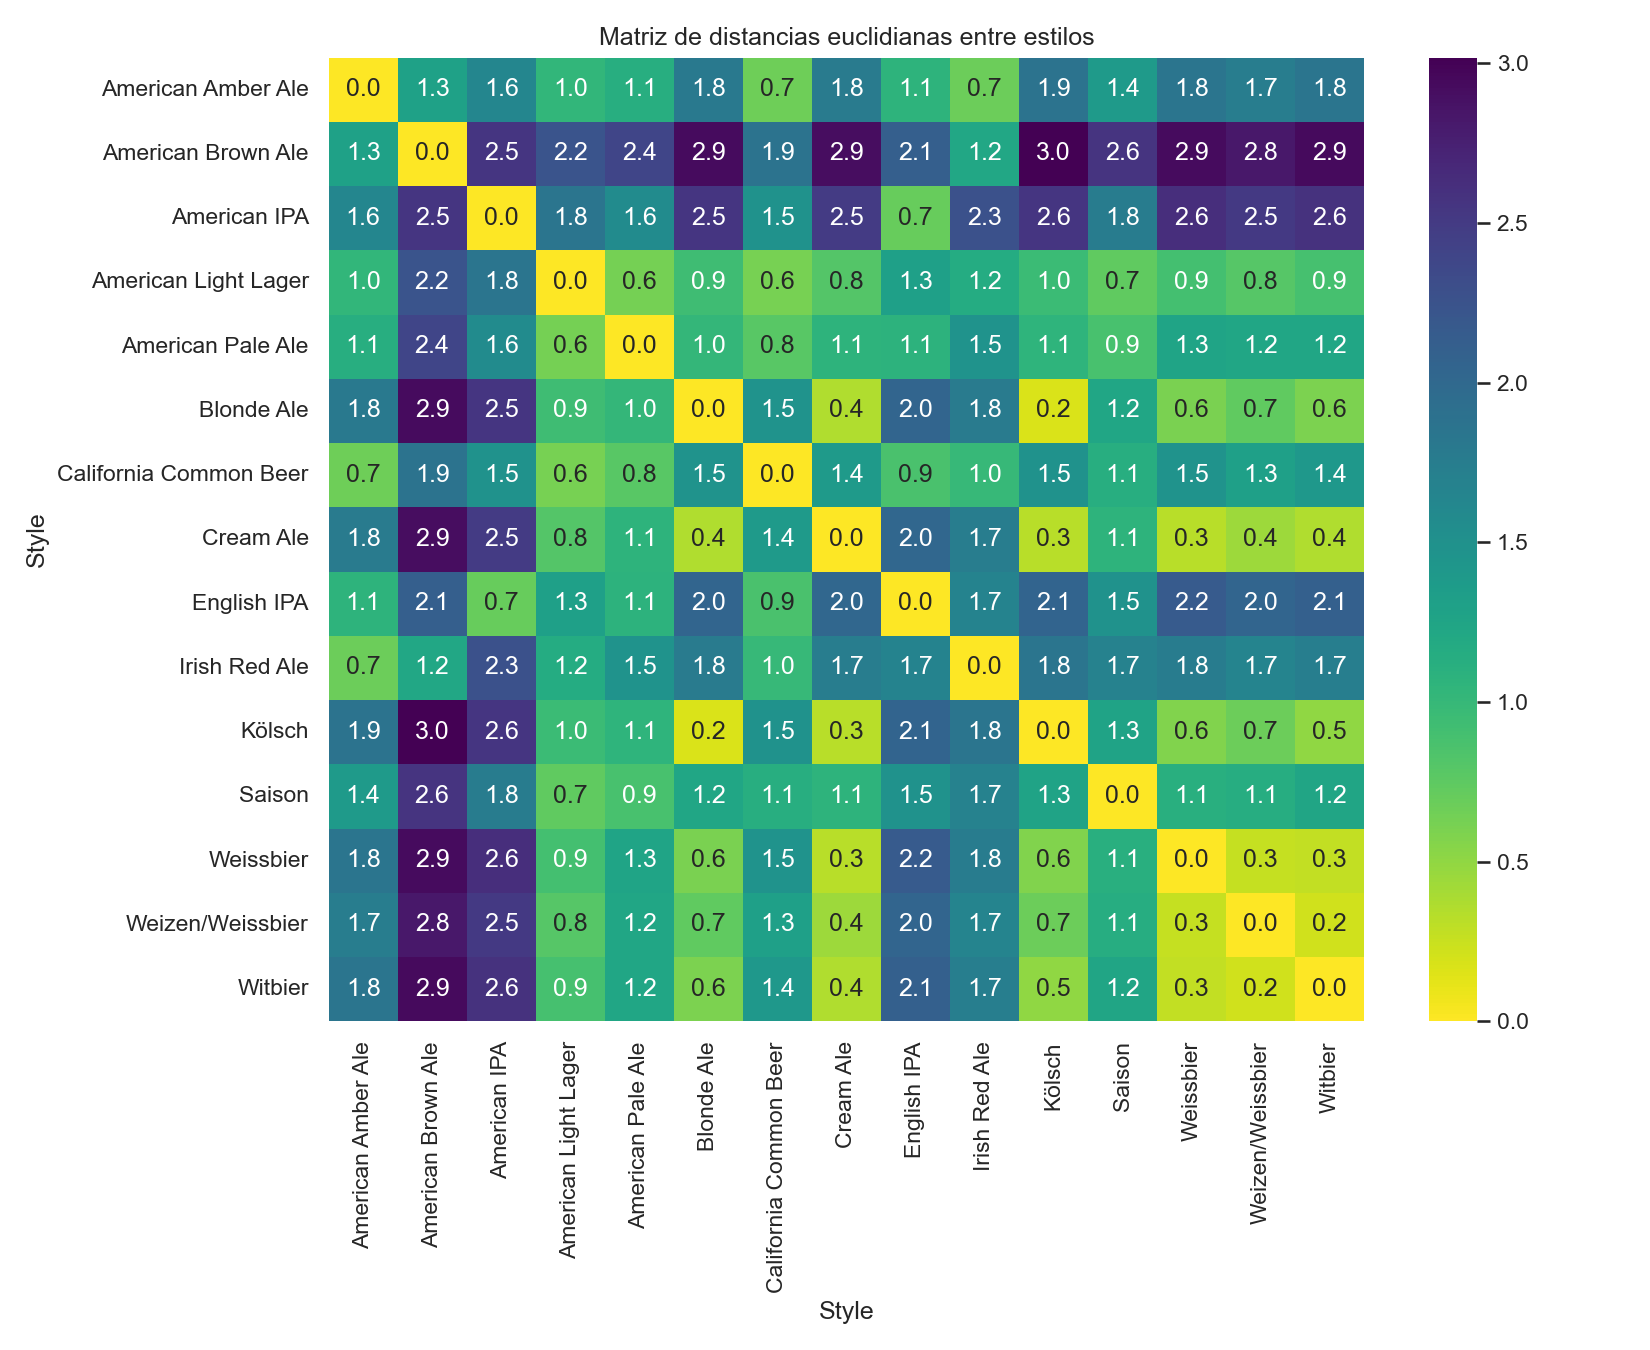
\includegraphics[width=0.85\textwidth]{figuras/dist_heatmap.png}
    \caption{Matriz de distancias euclidianas entre los 15 estilos más frecuentes.
    Los tonos más oscuros indican mayor parecido.}
    \label{fig:heatmap}
\end{figure}

\subsection{Correlación entre variables}

La Figura~\ref{fig:correlacion} muestra la matriz de correlación de Pearson. Los
resultados más relevantes son:
\begin{itemize}
    \item \textbf{ABV--OG: $r = 0.95$}, una correlación muy fuerte y positiva. Es
    coherente, ya que el azúcar inicial (OG) es lo que se convierte en alcohol al
    fermentar.
    \item \textbf{ABV--IBU: $r = 0.37$}, una relación positiva débil: las cervezas
    más fuertes tienden a ser ligeramente más amargas.
    \item \textbf{IBU--Color: $r = 0.02$}, prácticamente nula: el amargor y el
    color no están relacionados.
\end{itemize}

\begin{figure}[H]
    \centering
    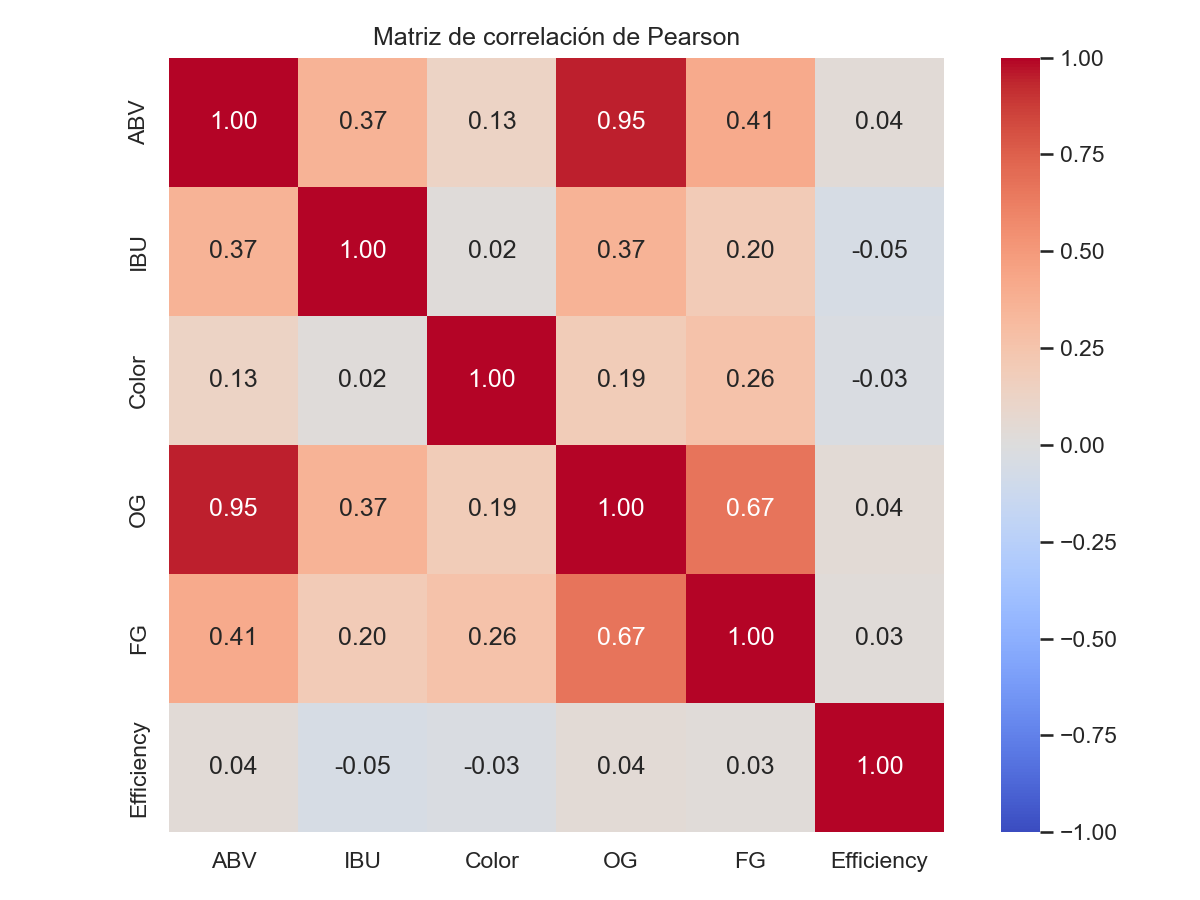
\includegraphics[width=0.6\textwidth]{figuras/correlacion.png}
    \caption{Matriz de correlación de Pearson entre las variables fisicoquímicas.}
    \label{fig:correlacion}
\end{figure}

\subsection{Prueba Chi-cuadrada}

La prueba Chi-cuadrada entre el estilo y el método de elaboración arrojó un
estadístico $\chi^2 = 74.17$ con un \textbf{valor $p = 1.3\times10^{-5}$}, menor a
$0.05$. Por lo tanto, se rechaza la hipótesis de independencia y se concluye que
\textbf{sí existe dependencia} entre el estilo de la cerveza y el método de
elaboración. Además, el $0\%$ de las celdas presentó una frecuencia esperada menor
a 5, por lo que se cumple el supuesto de la prueba y el resultado es confiable.

\subsection{Análisis de Componentes Principales (PCA)}

Las dos primeras componentes principales explican en conjunto el \textbf{61\% de la
varianza} (PC1: 43.8\%, PC2: 17.2\%). La primera componente (PC1) representa la
\textit{fuerza o cuerpo} de la cerveza (alcohol, densidades), mientras que la
segunda (PC2) contrapone el \textit{color} frente al \textit{amargor}. La variable
Efficiency no resultó relevante. Como se aprecia en la Figura~\ref{fig:pca}, los
estilos forman \textbf{grupos parcialmente identificables}: las cervezas oscuras
(como la \textit{American Brown Ale}) se ubican en la parte superior, mientras que
las claras y amargas (como la \textit{American IPA}) se sitúan en la parte
inferior, lo que coincide con el análisis de similitud.

\begin{figure}[H]
    \centering
    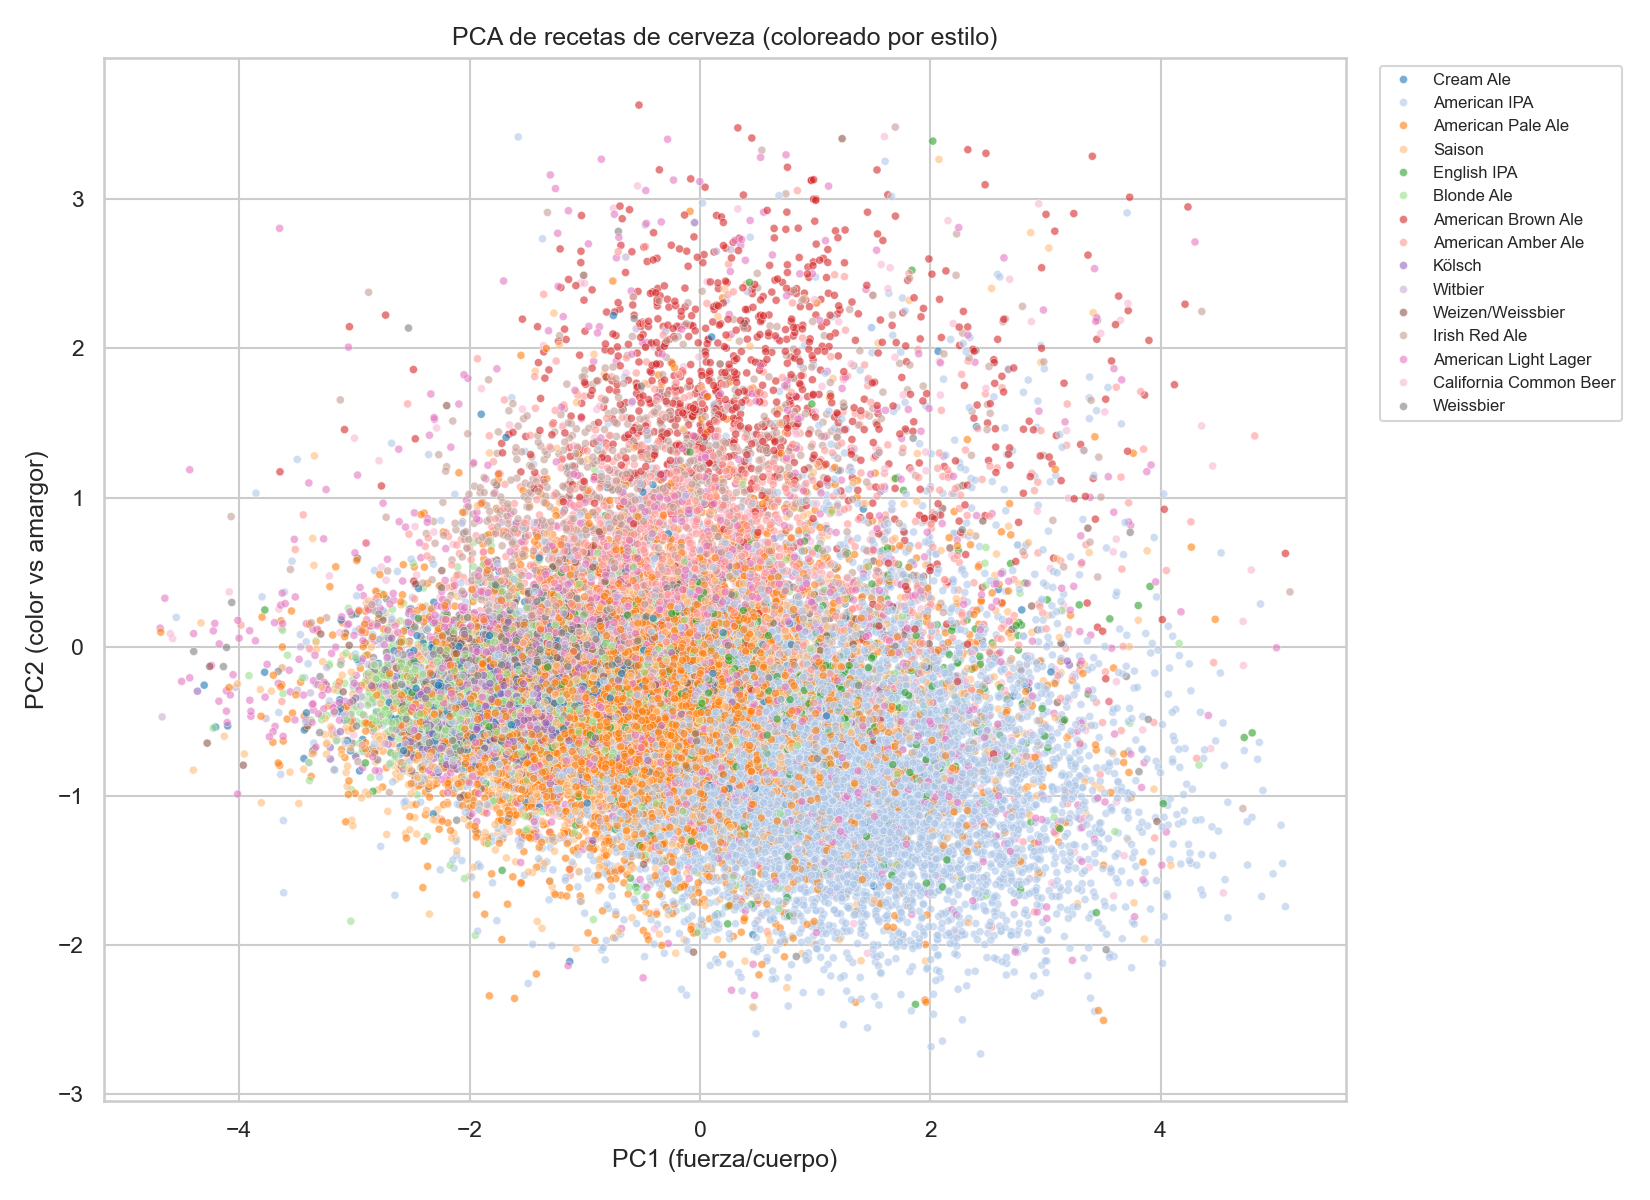
\includegraphics[width=0.85\textwidth]{figuras/pca.png}
    \caption{Representación de las recetas en las dos primeras componentes
    principales, coloreadas por estilo.}
    \label{fig:pca}
\end{figure}

\subsection{Dashboard}

Como resultado final se construyó un \textbf{dashboard interactivo} con las
herramientas \textit{Streamlit} (para la interfaz) y \textit{Plotly} (para las
gráficas). El dashboard lee el conjunto de datos ya limpio y permite explorar la
información sin necesidad de programar. Cuenta con una barra lateral de
\textbf{filtros} (estilo, método de elaboración y rangos de alcohol y amargor) que
actualizan todas las gráficas de forma automática, una fila de \textbf{indicadores
resumen} (número de recetas, estilos, ABV e IBU promedio) y la información
organizada en \textbf{pestañas}. A continuación se describe cada una de sus
secciones.

\textbf{1. Vista general y resumen.} Al abrir el dashboard se muestran los filtros,
los indicadores resumen y la pestaña \textit{Resumen}, que presenta la distribución
de los estilos de cerveza y los estilos más frecuentes de la selección actual
(Figura~\ref{fig:dash1}).

\begin{figure}[H]
    \centering
    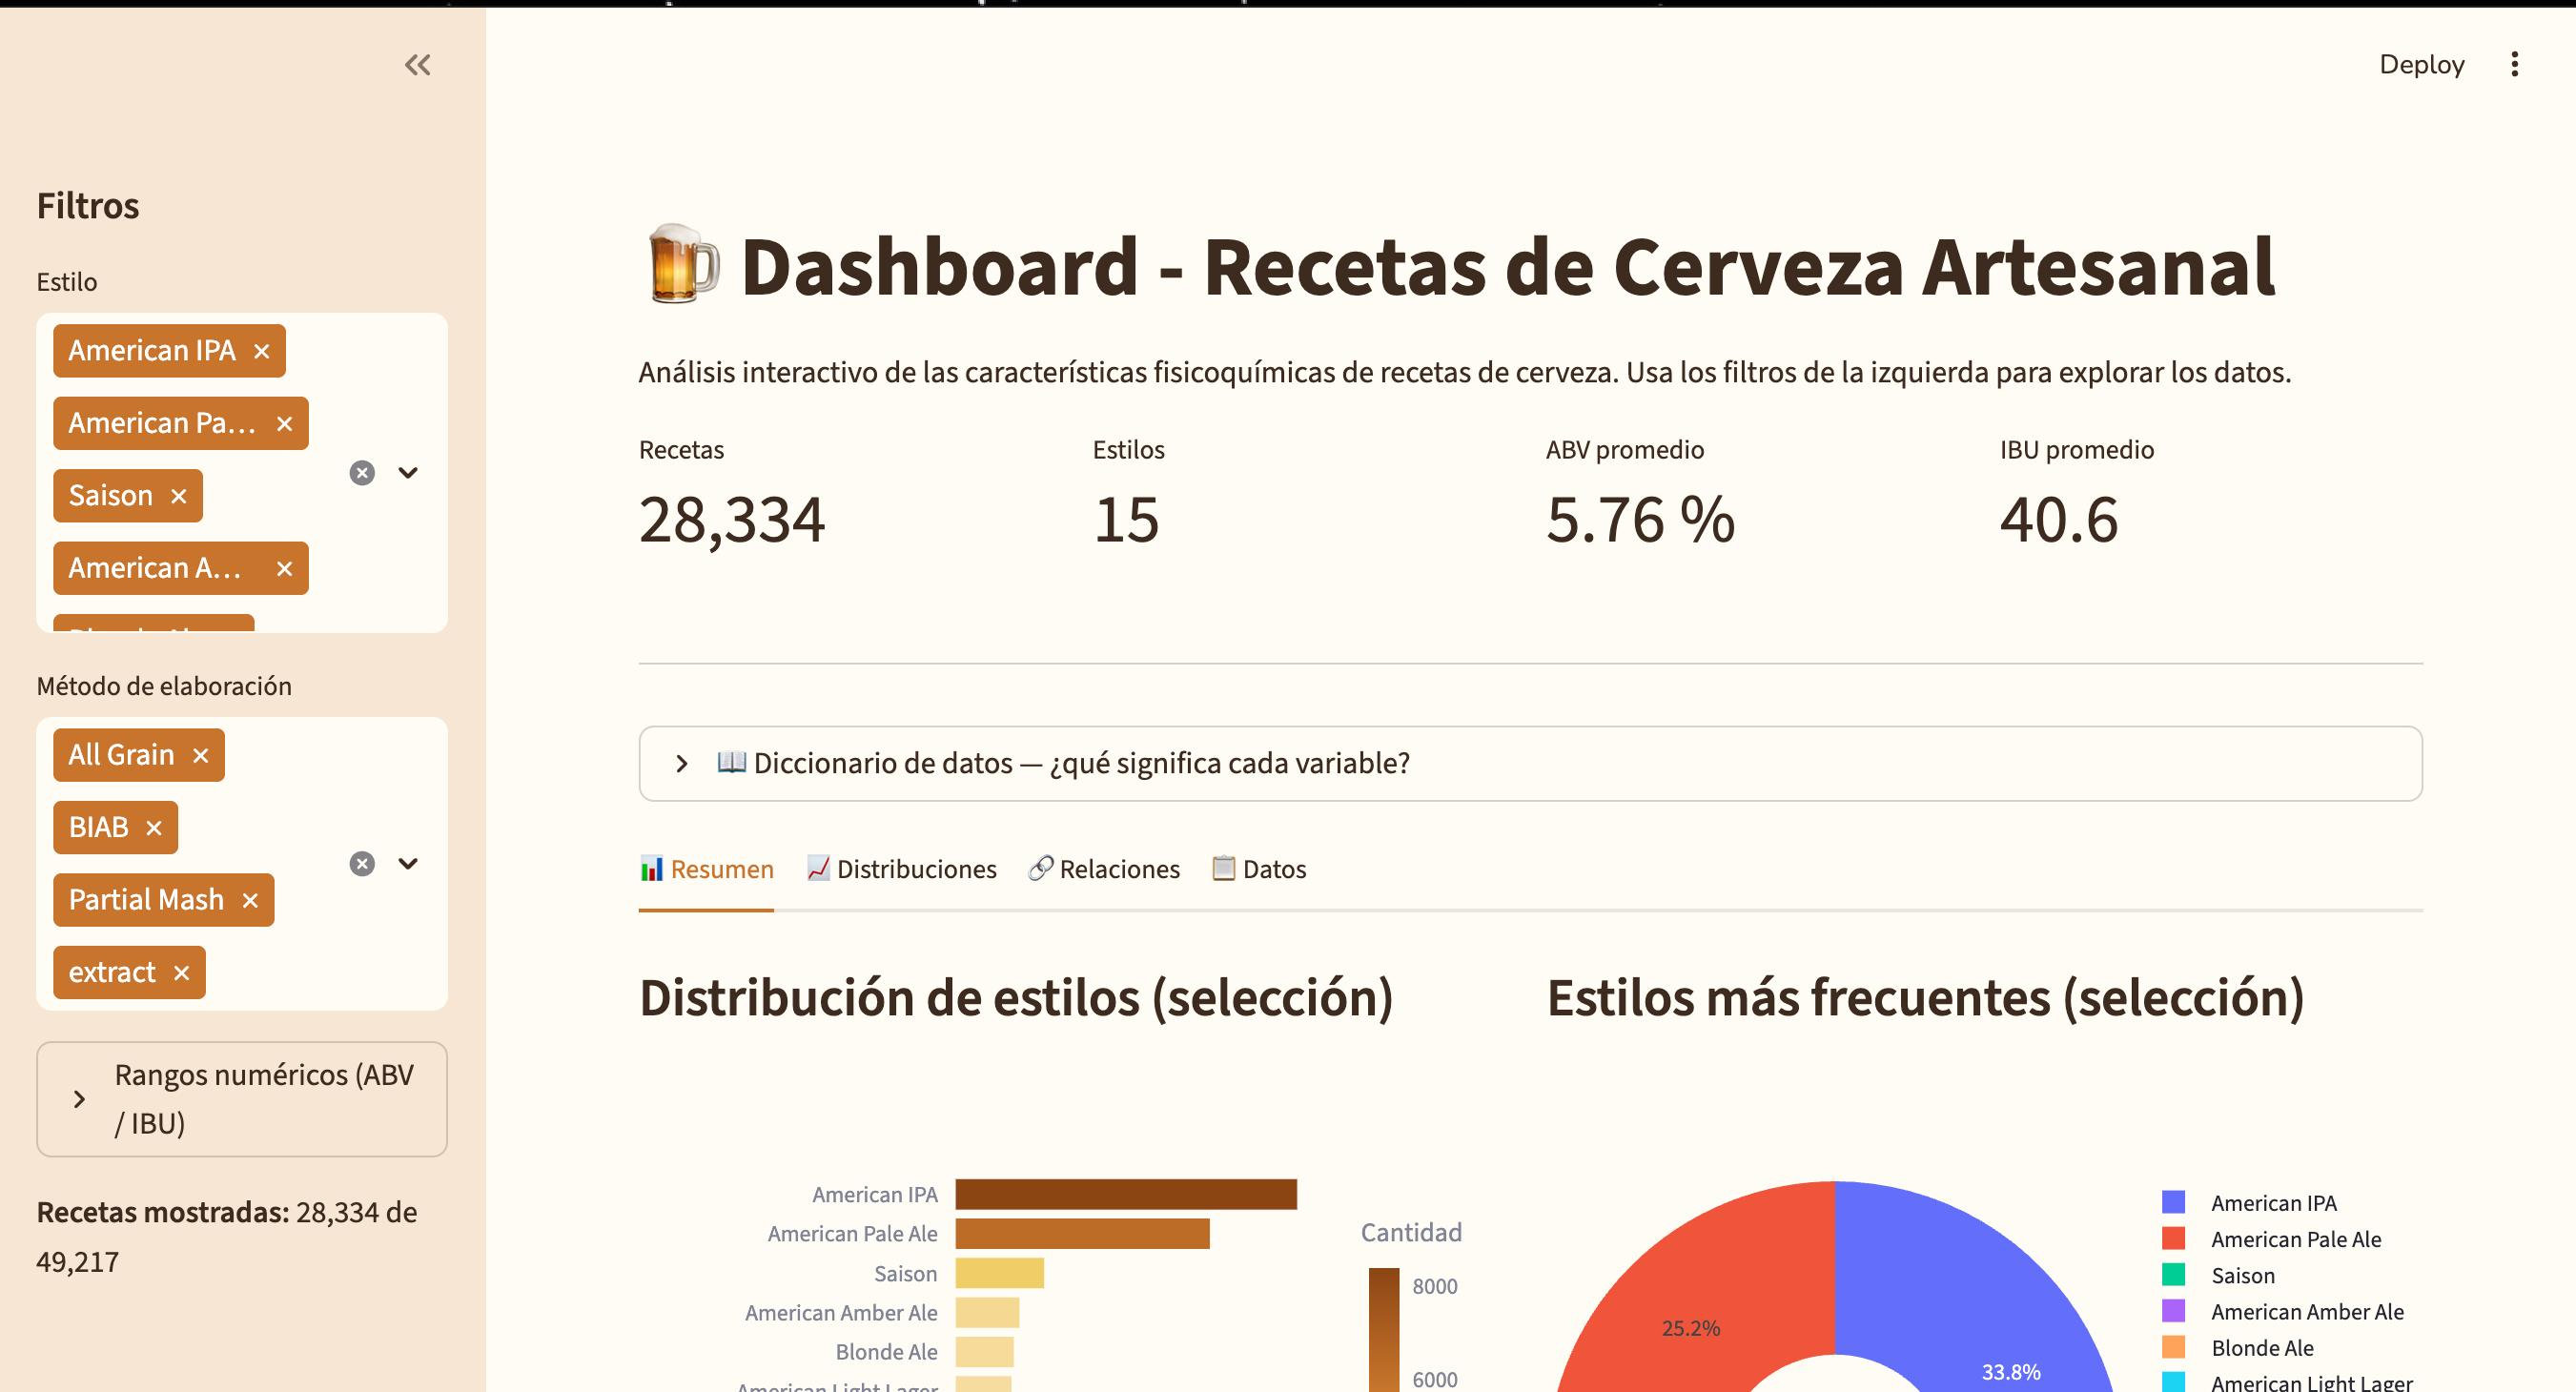
\includegraphics[width=0.9\textwidth]{figuras/dashboard1.jpeg}
    \caption{Vista general: filtros, indicadores resumen y distribución de estilos.}
    \label{fig:dash1}
\end{figure}

\textbf{2. Distribuciones.} La pestaña \textit{Distribuciones} muestra los
histogramas del alcohol (ABV) y del amargor (IBU), que permiten observar en qué
rangos se concentran la mayoría de las recetas (Figura~\ref{fig:dash2}).

\begin{figure}[H]
    \centering
    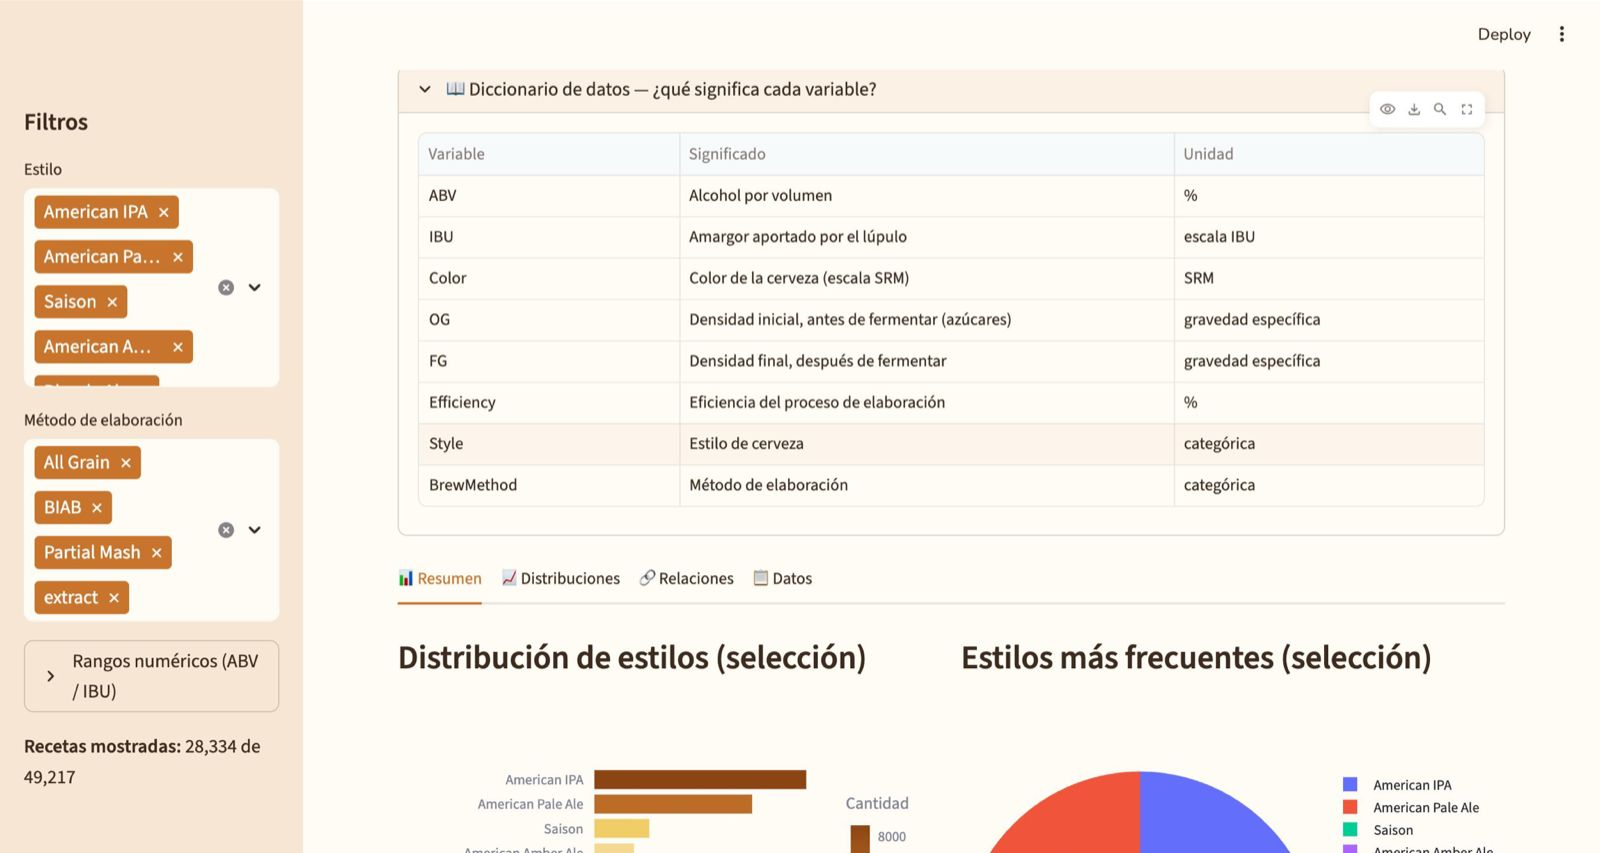
\includegraphics[width=0.9\textwidth]{figuras/dashboard2.jpeg}
    \caption{Pestaña de distribuciones: histogramas de ABV e IBU.}
    \label{fig:dash2}
\end{figure}

\textbf{3. Relaciones.} La pestaña \textit{Relaciones} permite comparar variables
mediante un diagrama de dispersión (en el que el usuario elige los ejes), además de
mostrar la proyección del PCA y la matriz de correlación (Figura~\ref{fig:dash3}).

\begin{figure}[H]
    \centering
    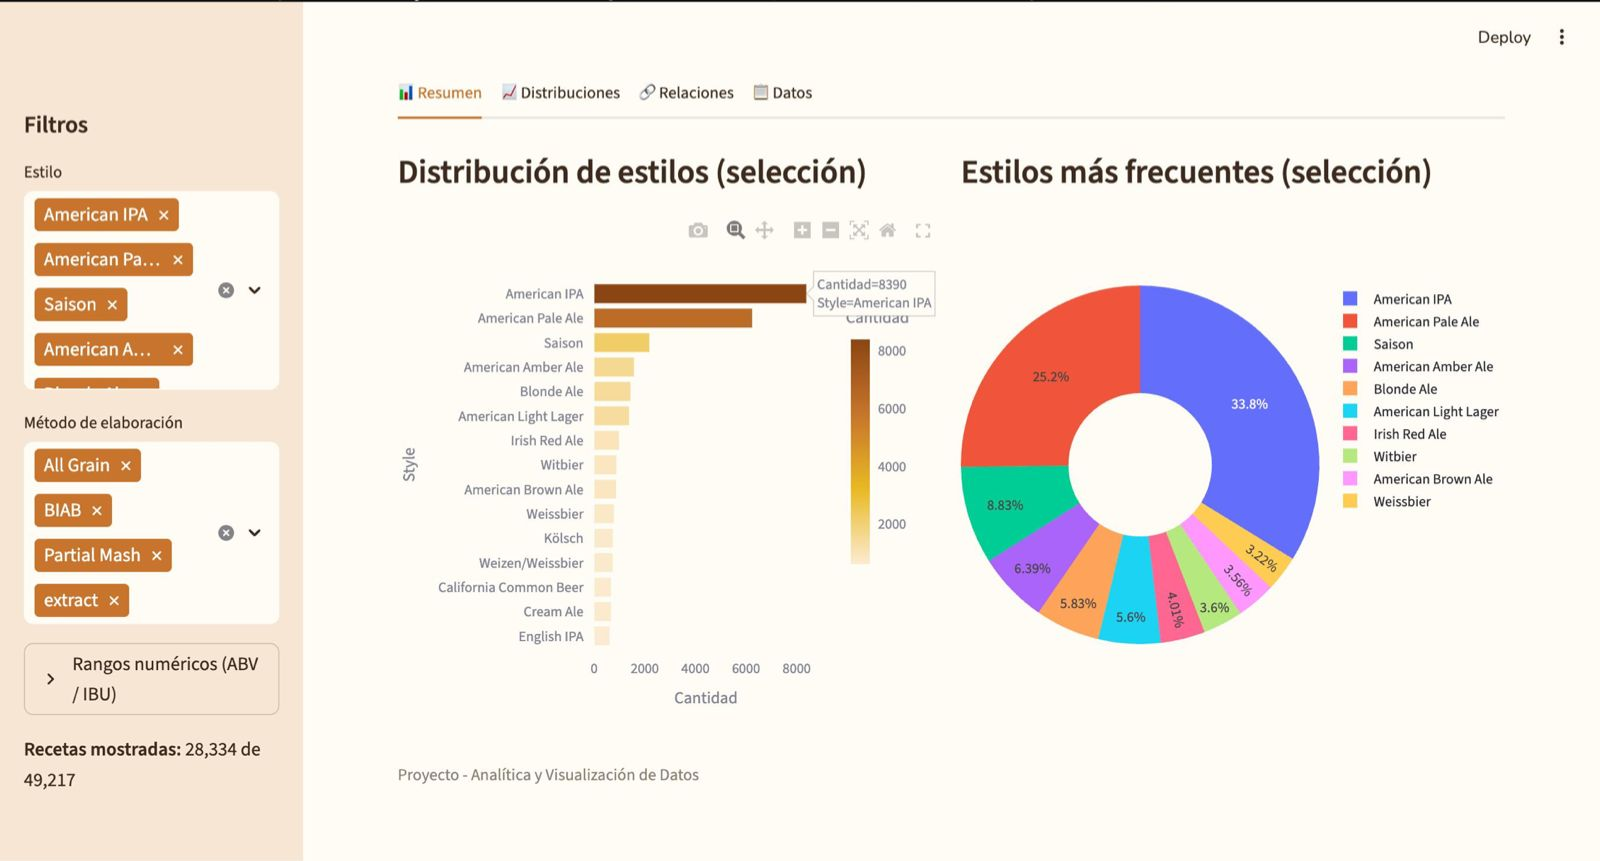
\includegraphics[width=0.9\textwidth]{figuras/dashboard3.jpeg}
    \caption{Pestaña de relaciones: dispersión entre variables, PCA y correlación.}
    \label{fig:dash3}
\end{figure}

\textbf{4. Datos.} La pestaña \textit{Datos} contiene un explorador de la tabla con
un buscador por estilo, que permite consultar las recetas individuales que cumplen
los filtros aplicados (Figura~\ref{fig:dash4}).

\begin{figure}[H]
    \centering
    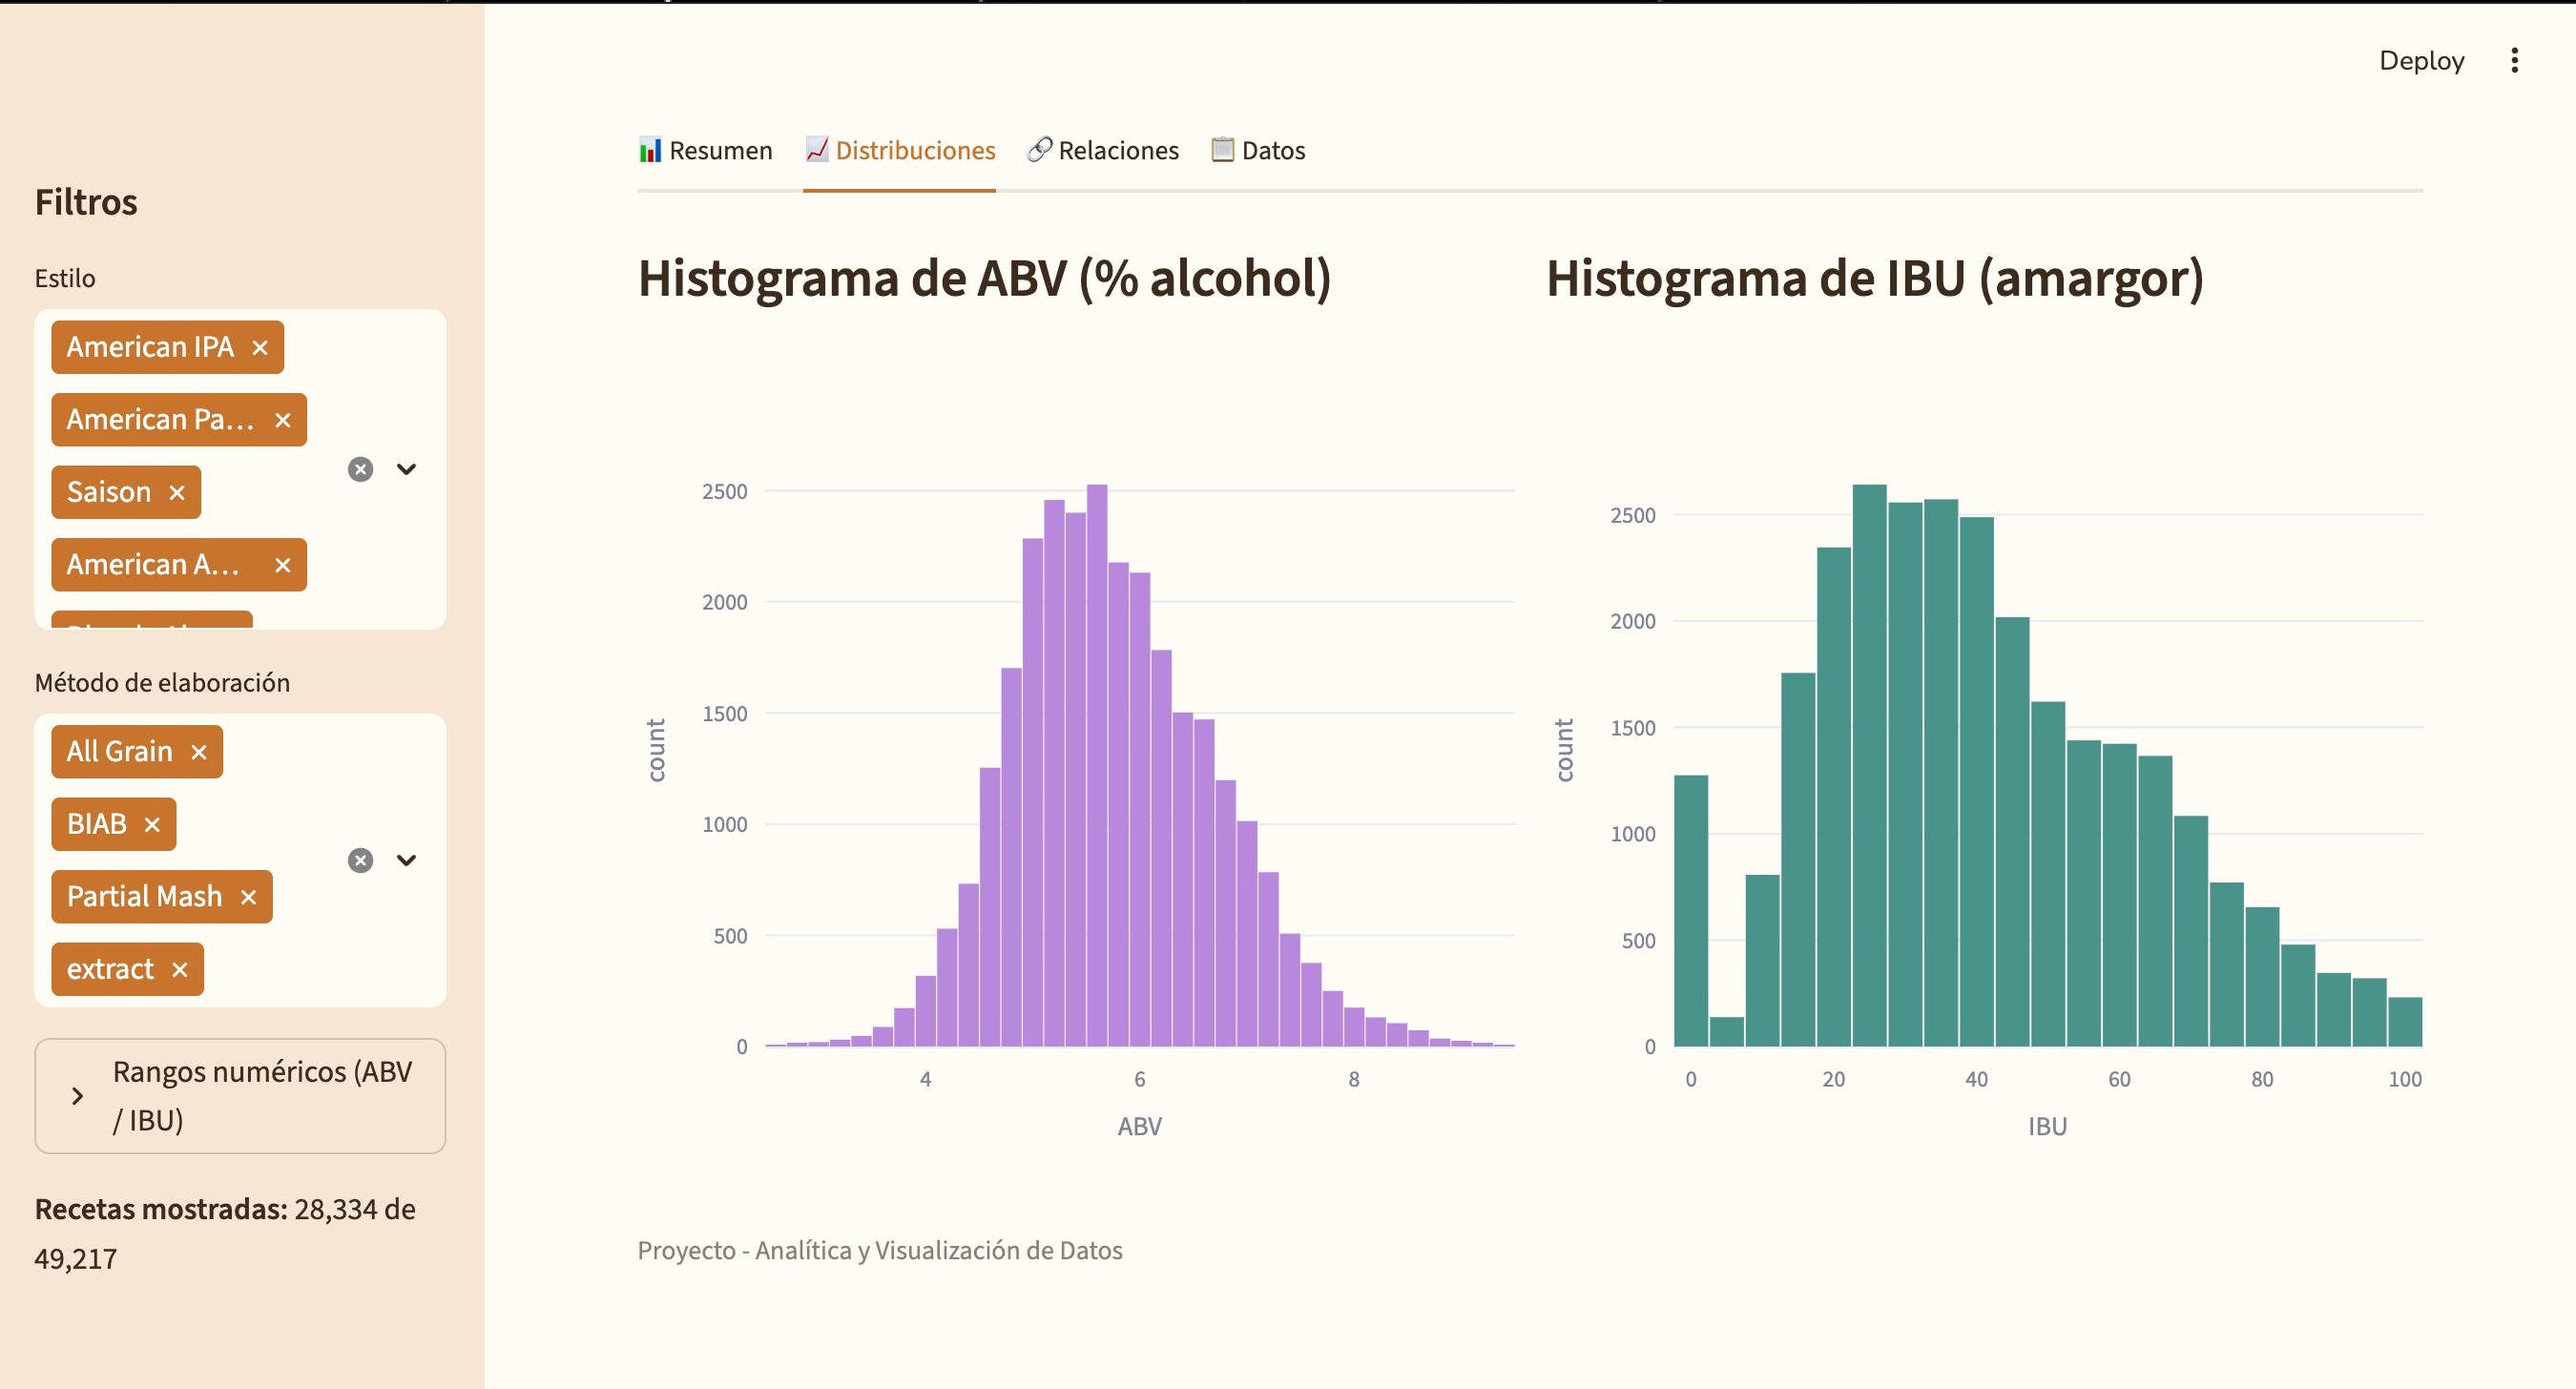
\includegraphics[width=0.9\textwidth]{figuras/dashboard4.jpeg}
    \caption{Pestaña de datos: explorador de la tabla con buscador.}
    \label{fig:dash4}
\end{figure}

\textbf{5. Diccionario de datos.} Por último, el dashboard incluye un panel
desplegable con el diccionario de datos, disponible en todo momento, que explica el
significado de cada variable (Figura~\ref{fig:dash5}).

\begin{figure}[H]
    \centering
    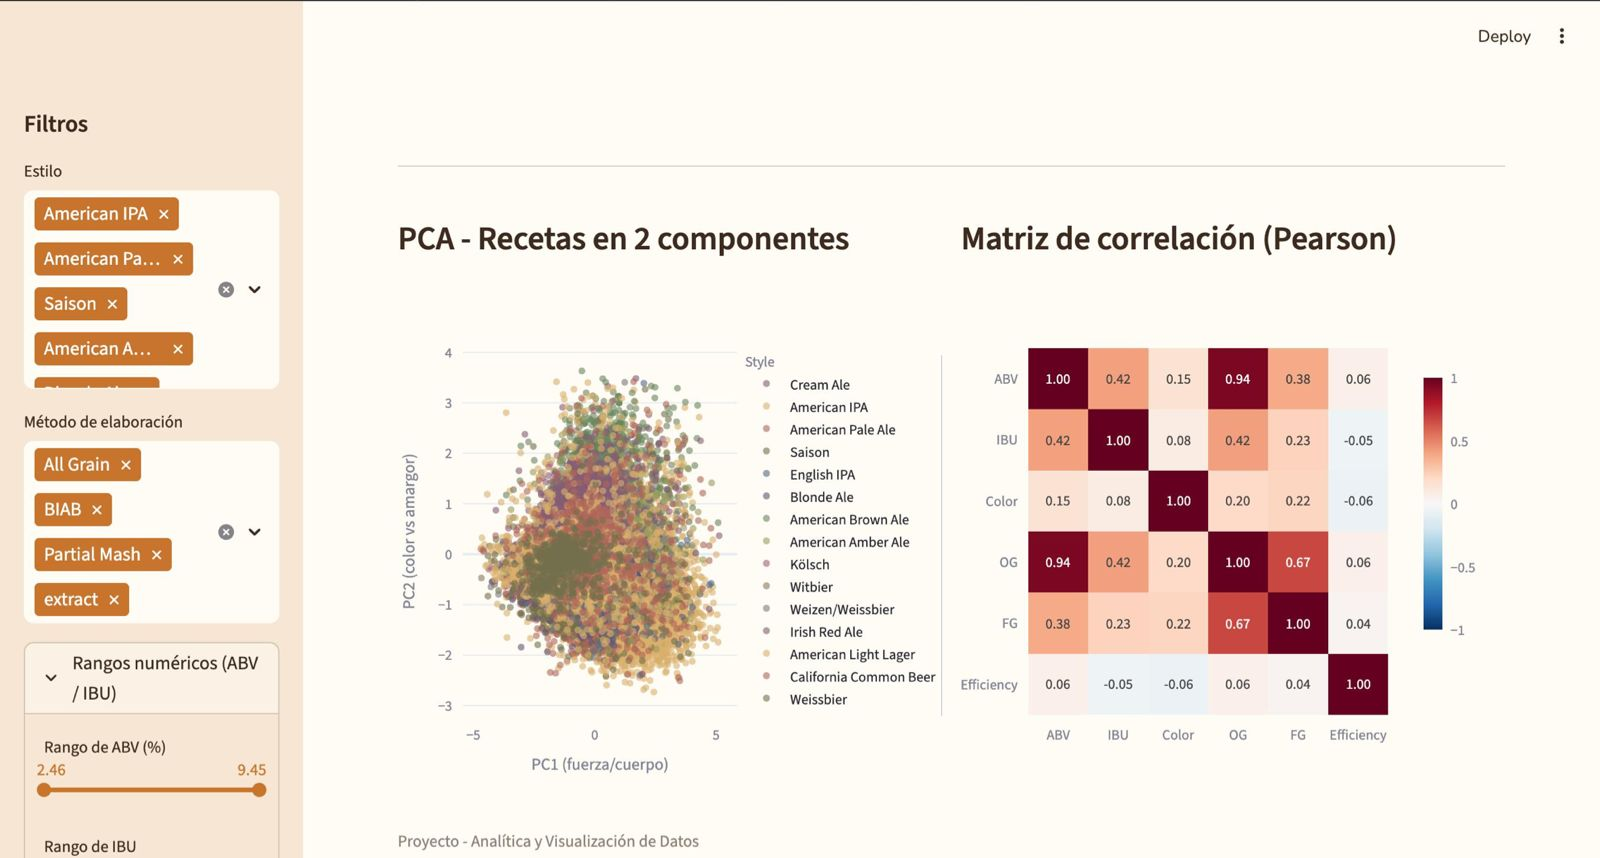
\includegraphics[width=0.9\textwidth]{figuras/dashboard5.jpeg}
    \caption{Diccionario de datos integrado en el dashboard.}
    \label{fig:dash5}
\end{figure}


% ============================================================
%  5. CONCLUSIONES
% ============================================================
\section{Conclusiones}

A lo largo de este proyecto se aplicó la metodología KDD, desde la limpieza de los
datos hasta su análisis y visualización, sobre un conjunto de más de 73{,}000
recetas de cerveza artesanal. El preprocesamiento permitió eliminar errores y
valores atípicos, reduciendo el conjunto a 49{,}217 recetas confiables y comparables
entre sí.

Un aspecto importante es que los distintos análisis realizados son coherentes, lo que da consistencia a los resultados. 
El análisis de similitud mostró que las cervezas claras y suaves (como la Blonde Ale y la Kölsch) se parecen
mucho entre sí, mientras que las cervezas oscuras y con más cuerpo (como la American
Brown Ale) se separan del resto. Esta misma agrupación se confirmó con el PCA, donde
los estilos forman grupos parcialmente identificables según su color, cuerpo y
amargor.

En cuanto a las relaciones entre variables, la correlación de Pearson reveló que el
alcohol depende casi por completo del azúcar inicial (ABV--OG, $r = 0.95$), mientras
que el amargor y el color resultaron independientes. Por su parte, la prueba
Chi-cuadrada confirmó que el estilo de la cerveza está relacionado con el método de
elaboración.

Finalmente, el dashboard interactivo permitió reunir todos estos hallazgos en una
sola herramienta visual, facilitando la exploración de los datos sin necesidad de
programar. En conjunto, este proyecto demuestra cómo aplicar técnicas de análisis de datos
para extraer conocimiento de un conjunto complejo, y cómo presentarlo de forma clara e interactiva.


% ============================================================
%  REFERENCIAS (opcional)
% ============================================================
\section*{Referencias}
\begin{itemize}
    \item Trofe, J. \textit{Beer Recipes Dataset} (Brewer's Friend). Kaggle.
    \url{https://www.kaggle.com/datasets/jtrofe/beer-recipes}
    \item Documentación de las bibliotecas \textit{pandas}, \textit{scikit-learn},
    \textit{SciPy}, \textit{Plotly} y \textit{Streamlit}.
\end{itemize}

\end{document}
